\documentclass[9pt,lineno,onehalfspacing]{elife}
% Use the onehalfspacing option for 1.5 line spacing
% Use the doublespacing option for 2.0 line spacing
% Please note that these options may affect formatting.
% Additionally, the use of the \newcommand function should be limited.

\usepackage{lipsum} % Required to insert dummy text
\usepackage[version=4]{mhchem}
\usepackage{siunitx}
\DeclareSIUnit\Molar{M}
\usepackage{amsmath}
\usepackage{threeparttable}

%%%%%%%%%%%%%%%%%%%%%%%%%%%%%%%%%%%%%%%%%%%%%%%%%%%%%%%%%%%%
%%% ARTICLE SETUP
%%%%%%%%%%%%%%%%%%%%%%%%%%%%%%%%%%%%%%%%%%%%%%%%%%%%%%%%%%%%
\title{Brief Report: Genomic epidemiology of a densely sampled COVID19 outbreak in China}

\author[1*]{Erik M Volz}
\author[1]{Han Fu}
\author[1]{Haowei Wang}
\author[2]{Xiaoyue Xi}


\author[3]{Wei Chen}
\author[3]{Dehui Liu}
\author[3]{Yingying Chen}
\author[3]{Mengmeng Tian}

\author[4]{Wei Tan}

\author[5]{Junjie Zai}

\author[6]{Wanying Sun}
\author[6]{Jiandong Li}
\author[6]{Junhua Li}

\author[7\authfn{1}\authfn{2}*]{Xingguang Li}

\author[3\authfn{1}\authfn{3}*]{Qing Nie}

\affil[1]{Department of Infectious Disease Epidemiology and MRC Centre for Global Infectious Disease Analysis, Imperial College London, Norfolk Place, W2 1PG, United Kingdom}
\affil[2]{Department of Mathematics, Imperial College London, London SW7 2AZ, United Kingdom}
\affil[3]{Department of Microbiology, Weifang Center for Disease Control and Prevention, Weifang 261061, China.}
\affil[4]{Department of Respiratory Medicine, Weifang People's Hospital, Weifang 261061, China.}
\affil[5]{Immunology Innovation Team, School of Medicine, Ningbo University, Ningbo 315211, China.}
\affil[6]{Shenzhen Key Laboratory of Unknown Pathogen Identification, BGI-Shenzhen, Shenzhen 518083, China.}
\affil[7]{Hubei Engineering Research Center of Viral Vector, Wuhan University of Bioengineering, Wuhan, 430415, China.}


\corr{nieqing0454@163.com}{QN}
\corr{xingguanglee@hotmail.com}{XL}

\contrib[\authfn{1}]{These authors contributed equally to this work}

\presentadd[\authfn{2}]{Department of Microbiology, Weifang Center for Disease Control and Prevention, Weifang 261061, China. Tel: +86-0536-8098503}
\presentadd[\authfn{3}]{Hubei Engineering Research Center of Viral Vector, Wuhan University of Bioengineering, Wuhan, 430415, China. Tel: +86-027-89648139}
% \presentadd[\authfn{5}]{eLife Sciences editorial Office, eLife Sciences, Cambridge, United Kingdom}

%%%%%%%%%%%%%%%%%%%%%%%%%%%%%%%%%%%%%%%%%%%%%%%%%%%%%%%%%%%%
%%% ARTICLE START
%%%%%%%%%%%%%%%%%%%%%%%%%%%%%%%%%%%%%%%%%%%%%%%%%%%%%%%%%%%%

\begin{document}

\maketitle

\begin{abstract}
%~ Please provide an abstract of no more than 150 words. Your abstract should explain the main contributions of your article, and should not contain any material that is not included in the main text.
Analysis of genetic sequence data from the pandemic SARS Coronavirus 2 can provide insights into epidemic origins, worldwide dispersal, and epidemiological history. With few exceptions, genomic epidemiological analysis has focused on geographically distributed data sets with few isolates in any given location. Here we report an analysis of 20 whole SARS-CoV 2 genomes from a single relatively small and geographically constrained outbreak in Weifang, People's Republic of China. 
Using Bayesian model-based phylodynamic methods, we estimate the reproduction number for the outbreak to be 2.6 (95\% CI:1.5-5). 
We further estimate the number of infections through time and compare these estimates to confirmed diagnoses by the Weifang Centers for Disease Control. 
We find that these estimates are consistent with reported cases and there is unlikely to be a large undiagnosed burden of infection over the period we studied. 
\end{abstract}


\section{Introduction}

We report a genomic epidemiological analysis of one of the first geographically concentrated community transmission samples of SARS-CoV 2 genetic sequences collected outside of the initial outbreak in Wuhan, China.
These data comprise 20 whole genome sequences from confirmed COVID19 infections in Weifang, Shandong Province, People’s Republic of China. 
The data were collected over the course of several weeks up to February 10, 2020 and overlap with a period of intensifying public health and social distancing measures. 
Phylodynamic analysis allows us to evaluate epidemiological trends after seeding events which took place in mid to late January, 2020. 

The objective of our analysis is to evaluate epidemiological trends based on national surveillance and response efforts by Weifang Centers for Disease Control (CDC). 
This analysis provides an estimate of the initial rate of spread and reproduction number in Weifang City. 
In contrast to the early spread of COVID19 in Hubei Province of China, most community transmissions within Weifang took place after public health interventions and social distancing measures were put in place. 
We therefore hypothesize that genetic data should reflect a lower growth rate and reproduction number than was observed in Wuhan. 
A secondary aim is to estimate the total numbers infected and to evaluate the possibility that there is a large unmeasured burden of infection due to imperfect case ascertainment and a large proportion of infections with mild or asymptomatic illness. 

To analyze the Weifang sequences, we have adapted model-based phylodynamic methods which were previously used to estimate growth rates and reproduction numbers using sequence data from Wuhan and exported international cases\citep{report5}.
This analysis has several constraints and requirements: \\
{\flushleft\it Importation of lineages from Wuhan.} The outbreak in Weifang was seeded by multiple lineages imported at various times from the rest of China. We use a  phylodynamic model that accounts for location of sampling. Migration is modeled as a bi-directional process with rates proportional to epidemic size in Weifang. The larger international reservoir of COVID19 cases serves as a source of new infections and is assumed to be growing exponentially over this period of time. 
{\flushleft\it Nonlinear epidemiological dynamics in Weifang.} The maximum number of daily confirmed COVID19 cases occurred on February 5, but it is unknown when the maximum prevalence of infection occurred. 
We use a susceptible-exposed-infectious-recovered (SEIR) model\citep{Keeling2011-wp} for epidemic dynamics in Weifang. 
The model accounts for a realistic distribution of generation times and can potentially capture a nonlinear decrease in cases following epidemic peak.
{\flushleft\it Variance in transmission rates\citep{Lloyd-Smith2005-oz}.}To estimate total numbers infected, the phylodynamic model must account for epidemiological variables which are known to significantly influence genetic diversity. 
Foremost among these is the variance in offspring distribution (number of transmissions per primary case). 
We draw on previous evidence based on the previous SARS epidemic which indicates that the offspring distribution is highly over-dispersed. 
High variance of transmission rates will reduce genetic diversity of a sample and failure to account for this factor will lead to highly biased estimates of epidemic size\citep{Li2017-mi}. 
Recent analyses of sequence data drawn primarily from Wuhan has found that high over-dispersion was required for estimated cases to be consistent with the epidemiological record\citep{report5}. 
Models assuming low variance in transmission rates between people would generate estimates of cases that are lower than the known number of confirmed cases. 
Separately, Grantz et al.\citep{Grantz_undated-ah} have found that high over-dispersion is required to reconcile estimated reproduction numbers with the observed frequency of international outbreaks. 
In this study, we elaborate the SEIR model to include a compartment($J$) with higher transmission rates. 
The variance of the implied offspring distribution is calibrated to give similar overdispersion from the SARS epidemic.


\section{Results}

Despite an initial rapid increase in confirmed cases in Weifang in late January and early February, the number of confirmed cases by Weifang CDC show that outbreak peaked quite early and maximum number of cases ocurred on February 5. 
Phylodynamic analysis supports the interpretation that control efforts reduced epidemic growth rates and contributed to eventual control. 
\FIG{fig1}A illustrates the phylodynamic model which was co-estimated with the phylogeny which provides estimates of epidemiological parameters summarized in \TABLE{tab1}.
\FIG{fig1}B shows the estimated time scaled phylogeny (maximum clade credibility) including 20 lineages sampled from distinct patients in Weifang and 33 genomes sampled from Wuhan and internationally. 


The estimated number of infections is shown Figure \ref{fig:fig1}C.
The time series of confirmed cases should lag the estimated number of infected because of delays from infection to appearance of symptoms and delays from symptoms to diagnosis. 
We also expect that an unknown proportion of infections will be missed by the surveillance system due very mild, subclinical, or asymptomatic infection. 
Our estimates do not support the hypothesis that there was a very large hidden burden of infection in Weifang over the period that the sequence data were sampled. 
Indeed, our central estimate for the number infected on 10th February is only 142 and the credible intervals cover the 44 cumulative confirmed cases at the end of February. 
%~ 1.422042e+02 4.322300e+00 1.692355e+03




\begin{figure}
\begin{fullwidth}
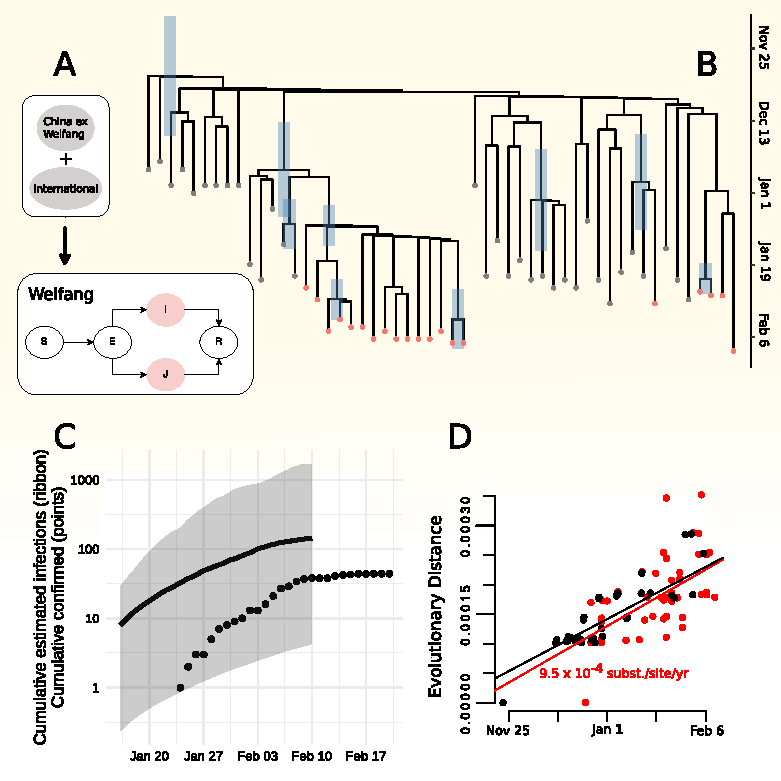
\includegraphics[width=.9\linewidth]{fig1_2.pdf}
\caption{ Phylodynamic estimates and epidemiological model. A. Diagram representing the structure of the epidemiological SEIR model which was fitted in tandem with the time scaled phylogeny. Colours correspond to the state of individuals sampled and represented in the tree (B). Note that infected and infectious individuals may occupy a low transmission state (I) or a high transmission rate state (J) to account for high dispersion of the reproduction number. B. A time scaled phylogeny co-estimated with epidemiological parameters. The colour of tips corresponds to location sampling. Red tips were sampled from Weifang, China. The credible interval of TMRCA is shown as a blue bar for all nodes with more than 50\% posterior support. C. Cumulative estimated infections through time produced by fitting the SEIR model and the cumulative confirmed cases (points) reported by Weifan CDC. The shaded region shows the 95\% HPD and the line shows the posterior median. D. A root to tip regression showing approximately linear increase in diversity with time of sampling. 
}
\label{fig:fig1}
\figsupp[Maximum likelihood time tree.]{A time scaled phylogeny estimated using IQTree and treedater and using the same data as used for the Bayesian analysis.}{\includegraphics[width=.5\textwidth]{treedatertree.pdf}}\label{figsupp:treedater}
\figsupp[Tree posterior density plot.]{A tree density plot based on the posterior distribution of trees computed in BEAST2. }{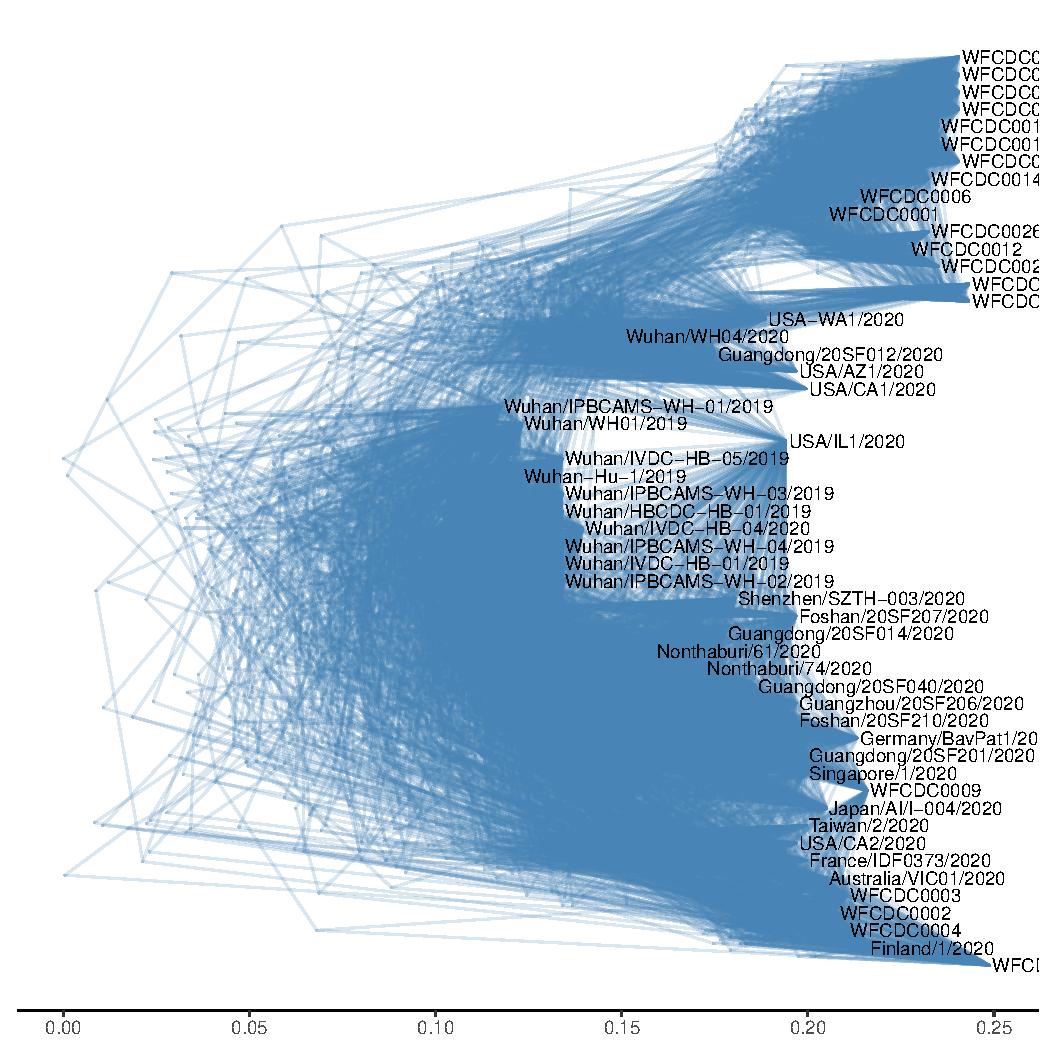
\includegraphics[width=.9\textwidth]{densitree.pdf}}\label{figsupp:densitree}
\figsupp[Tree posterior density plot.]{The estimated posterior TMRCA among all Weifang lineages.}{\includegraphics[width=6cm]{wftmrca2.pdf}}\label{figsupp:wftmrca}
\end{fullwidth}
\end{figure}



\begin{table}[ht]
\begin{fullwidth}
\begin{threeparttable}[b]
\caption{Summary of primary epidemiological and evolutionary parameters, including Bayesian prior distributions and estimated posteriors. Posterior uncertainty is summerized using a 95\% highest posterior density interval. \label{tab:tab1}}
\centering
\begin{tabular}{lllll}
  \hline
 & {\bf Parameter} & {\bf Prior} & {\bf Posterior mean} & \bf{95\% HPD} \\ 
  \hline
 & Initial infected & Exponential(mean=1) & 4.5 & 0.26-13 \\ 
 & Initial susceptible & Log-normal(mean log=6, sd log=1) & 660 & 23-3000 \\ 
 & Migration rate\tnote{1} & Exponential(mean=10*) & 1.6 & 0.73-2 \\ 
 & Reproduction number & Log-normal(mean log=1.03, sd log =0.5) & 2.6 & 1.5-5 \\ 
 & Molecular clock rate\tnote{2} & Uniform(0.0007,0.003) & 0.00098 & 0.00071-0.0015 \\ 
 & Transition/transversion & Log-normal(mean log=1,sd log=1.25) & 5.5 & 3.1-9.4 \\ 
 & Gamma shape & Exponential(mean=1) & 0.74 & 0.015-3 \\ 
   \hline
\end{tabular}
\begin{tablenotes}\item [1] Units: Migrations per lineage per year. \end{tablenotes}
\begin{tablenotes}\item [2] Units: Substitutions per site per year. \end{tablenotes}
\end{threeparttable}
\end{fullwidth}
\end{table}

We do not have sufficient data to detect a large decrease in epidemic growth rates as the epidemic progressed.
We estimate $R_0=2.6$ (95\% HPD:1.5-5). The growth rate in estimated infections remained positive but decreased substantially over the sampling period. 
These estimates correspond to growth during a period when Weifang was implementing a variety of public health interventions and contact tracing to limit epidemic spread.
These interventions included public health messaging, establishing phone hotlines, encouraging home isolation for recent vitors from Wuhan (January 23-26), optimizing triage of suspected cases in hospitals (January 24), travel restrictions(January 26), extending school closures, and establishing `fever clinics' for consulatation and diagnosis(January 27)\citep{Mao2020-qu}. 

As well as providing novel epidemiological estimates, our results point to the significance of realistic modeling for fidelity of phylogenetic inference.
The use of a model-based structured coalescent prior had large influence over estimated molecular clock rates and inferred TMRCAs. 
\FIGSUPP{treedater} shows that maximum likelihood inference of time-scaled phylogenies produces a distribution of TMRCAs which are substantially different than the Bayesian model-based analysis.
Choice of population genetic prior will have a large influence on phylogenetic inference based on sparse or poorly informative genetic sequence data. 
Among the 20 Weifang sequences included in this analysis, there is mean pairwise difference of only three single nucleotide polymorphisms and only approximately twice as much diversity observed among the remainder of the sequences we studied. 
There is correspondingly low confidence in tree topology (\FIGSUPP{densitree}), and only three clades had greater than 50\% posterior support including one clade which had a monophyletic compoisition of 13 Weifang lineages. 
The earliest Weifang sequence was sampled on January 25 from a patient who showed first symptoms on January 16. These dates cover a similar range as the posterior TMRCA of all Weifang sequences (\FIGSUPP{wftmrca}).


\section{Discussion}

Our analysis of 20 SARS-CoV 2 genomes from Weifang, China has confirmed independent observations regarding the rate of spread and burden of infection in the city.
Surveillance of COVID19 is rendered difficult by high proportions of illness with mild severity and an unknown proportion of asymptomatic infection\citep{Guan2020-ql}. 
The extent of under-reporting and case ascertainment rates has been widely debated. 
Analysis of genetic sequence data provides an alternative source of information about epidemic size which can be more robust to imperfect case ascertainment. 
We do not find evidence for a very large hidden burden of infection within Weifang. 
The relatively low estimate of $R_0$ is consistent with a slower rate of spread outside of Wuhan and effective control strategies implemented in late January. 


While the value of pathogen genomic analyses is widely recognized for estimating dates of emergence\citep{Verity_Hill2020-uf,Gire2014-ql} and identifying animal reservoirs\citep{Zhou2020-pi,Dudas2018-ht}, analysis of pathogen sequences also has potential to inform epidemic surveillance and intervention efforts. 
With few exceptions \citep{stadler_2020-yc,Bedford2020-zl}, this potential is currently not being realized for the international response to COVID19. 
It is worth noting that the analysis described in this report was accomplished in approximately 48 hours and drew on previously developed models and packages for BEAST2\citep{bouckaert2019beast,Volz2018-mm}. 
It is therefore feasible for phylodynamic analysis to provide a rapid supplement to epidemiological surveillance, however this requires rapid sequencing and timely sharing of data as well as randomized concentrated sampling of the epidemic within localities such as individual cities. 

\section{Methods and Materials} 

{\flushleft\bf Epidemiological investigation, sampling, and genetic sequencing.}
As of 10 February 2020, 136 suspected cases, and 214 close contacts were diagnosed by
Weifang Center for Disease Control and Prevention. 28 cases were detected positive with
SARS-CoV-2. Viral RNA was extracted using Maxwell 16 Viral Total Nucleic Acid
Purification Kit (Promega AS1150) by magnetic bead method and RNeasy Mini Kit
(QIAGEN 74104) by column method. RT-qPCR was carried out using 2019 novel
coronavirus nucleic acid detection kit (BioGerm, Shanghai, China) to confirm the presence of
SARS-CoV-2 viral RNA with cycle threshold (Ct) values range from 17 to 37, targeting the
high conservative region (ORF1ab/N gene) in SARS-CoV-2 genome.
Metagenomic sequencing:
The concentration of RNA samples was measurement by Qubit RNA HS Assay Kit (Thermo
Fisher Scientific, Waltham, MA, USA). DNase was used to remove host DNA. The
remaining RNA was used to construct the single-stranded circular DNA library with
MGIEasy RNA Library preparation reagent set (MGI, Shenzhen, China). Purified RNA was
then fragmented. Using these short fragments as templates, random hexamers were used to
synthesize the first-strand cDNA, followed by the second strand synthesis. Using the short
double-strand DNA, a DNA library was constructed through end repair, adaptor ligation, and
PCR amplification. PCR products were transformed into a single strand circular DNA library
through DNA-denaturation and circularization. DNA nanoballs (DNBs) were generated with
the single-stranded circular DNA library by rolling circle replication (RCR). The DNBs were
loaded into the flow cell and pair-end 100bp sequencing on the DNBSEQ-T7 platform 8
(MGI, Shenzhen, China).
20 genomes were assembled with length from 26,840 to 29,882 nucleotides.
%~ , and coverage depth ranged from XXXXXX to XXXXXX. 
The median age of patients was 36 (range:6-75). Two of twenty patients suffered severe or critical illness. 
Weifang sequences were combined with a diverse selection of sequences from China outside of Weifang and other countries provided by GISAID\cite{elbe2017data}. 
The new Weifang sequences are deposited in GISAID (EPI\_ISL\_413691, EPI\_ISL\_413692, EPI\_ISL\_413693, EPI\_ISL\_413694, EPI\_ISL\_413695, EPI\_ISL\_413696, EPI\_ISL\_413697, EPI\_ISL\_413711, EPI\_ISL\_413729, EPI\_ISL\_413746, EPI\_ISL\_413747, EPI\_ISL\_413748, EPI\_ISL\_413749, EPI\_ISL\_413750, EPI\_ISL\_413751, EPI\_ISL\_413752, EPI\_ISL\_413753, EPI\_ISL\_413761, EPI\_ISL\_413791, EPI\_ISL\_413809). 
%~ ((Elbe, S. & Buckland-Merrett, G. Data, disease and diplomacy: GISAID's innovative contribution to global health. Glob Chall1, 33-46, doi:10.1002/gch2.1018 (2017) )



{\flushleft\bf Mathematical model.} The phylodynamic model is designed to account for nonlinear epidemic dynamics in Weifang, a realistic course of infection (incubation and infectious periods), migration of lineages in and out of Weifang, and variance in transmission rates which can influence epidemic size estimates. 
The model of epidemic dynamics within Weifang is based on a susceptible-exposed-infectious-recovered (SEIR) model. 
We elaborate the model with with an additional compartment $J$ which has a higher transmission rate ($\tau$-fold higher) than the $I$ compartment. 
Upon leaving the incubation period individuals progress to the $J$ compartment with probability $p_h$, or otherwise to $I$. 
The model is implemented as a system of ordinary differential equations:
\begin{align}
\dot{S}(t) &= - \beta \left( \beta I(t) + \beta \tau J(t) \right)  \frac{S(t)}{S(t) + I(t) + J(t) + R(t)} \\  
\dot{E}(t) &= \beta \left( \beta I(t) + \beta \tau J(t) \right)  \frac{S(t)}{S(t) + I(t) + J(t) + R(t)} - \gamma_0 E(t) \\  
\dot{I}(t) &= \gamma_0 (1-p_h) E(t) - \gamma_1 I(t) \\
\dot{J}(t) &= \gamma_0 p_h E(t) - \gamma_1 J(t)  \\
\dot{R}(t) &= \gamma_1 (E(t) + J(t) )  
\end{align}

We also model an exponentially growing reservoir $Y(t)$ for imported lineages in to Weifang. 
The equation governing this population is 
\begin{align}
\dot{Y}(t) &= (\rho - \mu) Y(t).
\end{align}

Migration is modeled as a bidirectional process which only depends on the size of variables in the Weifang compartment and thus migration does not influence epidemic dynamics; it will only influence the inferred probability that a lineage resides within Weifang. 
For a compartment $X$ (E,I, or J), $\eta$ is the per lineage rate of migration out of Weifang and the total rate of migration in and out of Weifang is $ \eta X $. 

During phylodynamic model fitting $\beta$ and $\rho$ are estimated. 
Additionally, we estimate initial sizes of $Y$, $E$, and $S$. 
Other parameters are fixed based on prior information. We fix $1/\gamma_0=4.1$days and $1/\gamma_1=3.8$ days. 
We set $p_h=0.20$ and $\tau=74$ which yields a dispersion of the reproduction number that matches a negative binomial distribution with $k=0.22$ if $R_0=2$, similar to values estimated for the 2003 SARS epidemic \citep{Lloyd-Smith2005-oz}.  %TODO ref for incubation 



{\flushleft\bf Phylogenetic analysis.} We aligned the 20 Weifang sequences using MAFFT\citep{katoh2013mafft} with a previous aligment of 35 SARS-CoV 2 sequences from outside of Weifang\citep{report5}. 
Maximum likelihood analysis was carried using IQTree\citep{Minh2019-bp} with a HKY+G4 substitution model and a time-scaled tree was estimated using treedater 0.5.0\citep{Volz2017-nz}. 
Two outliers according to the molecular clock model were identified and removed using `treedater' which was also used to compute the root to tip regression. 

Bayesian phylogenetic analysis was carried out using BEAST 2.6.1\citep{bouckaert2019beast} using a HKY+G4 substitution model and a strict molecular clock.
The phylodynamic model was implemented using the PhyDyn package\citep{Volz2018-mm} using the QL likelihood approximation and the RK ODE solver. 
The model was fitted by running 8 MCMC chains in parallel and combining chains after removing 50\% burn-in. 

The \emph{ggtree} package was used for all phylogeny visualizations\citep{Yu2017-iy}.

Code to replicate this analysis and and BEAST XML files can be found at \url{https://github.com/emvolz/weifang-sarscov2}. 

\section{Funding} %funding statement should not go in submitted version 

This work was supported by Centre funding from the UK Medical Research Council under a concordat with the UK Department for International Development. NIHR. J-IDEA. This work was also supported by a grant from the Special Project for Prevention and Control of Pneumonia of New Coronavirus Infection in Weifang Science and Technology Development Plan in 2020 (2020YQFK015) to Associate Senior Technologist Qing Nie. 
Role of the Funders:  All funders of the study had no role in study design, data analysis, data interpretation, or writing of the report.


\section{Acknowledgements}

We gratefully acknowledge China National GeneBank at Shenzhen, China for the sequencing strategy and capacity support. We also gratefully  acknowledge  the  laboratories  that  have  contributed  publicly  available  genomes  via GISAID: Shanghai Public Health Clinical Center \& School of Public Health, Fudan University, Shanghai, China, at the National Institute for Viral Disease Control and Prevention, China CDC, Beijing, China, at the  Institute  of  Pathogen  Biology,  Chinese  Academy  of  Medical  Sciences  \&  Peking  Union  Medical College,  Beijing,  China,  at  the  Wuhan  Institute  of  Virology,  Chinese  Academy  of  Sciences,  Wuhan, China,  at  the  Department  of  Microbiology,  Zhejiang  Provincial  Center  for  Disease  Control  and Prevention, Hangzhou, China, at the Guangdong Provincial Center for Diseases Control and Prevention at the Department of Medical Sciences, at the Shenzhen Key Laboratory of Pathogen and Immunity, Shenzhen, China, at the Hangzhou Center for Disease and Control Microbiology Lab, Zhejiang, China, at  the  National  Institute  of  Health,  Nonthaburi,  Thailand,  at  the  National  Institute  of  Infectious Diseases,  Tokyo, Japan, at the Korea Centers  for Disease  Control \&  Prevention, Cheongju, Korea, at the  National  Public  Health  Laboratory,  Singapore,  at  the  US  Centers  for  Disease  Control  and  Prevention,  Atlanta,  USA,  at  the  Institut  Pasteur,  Paris,  France,  at  the  Respiratory  Virus  Unit, Microbiology Services Colindale, Public Health England, and at the Department of Virology, University of  Helsinki  and  Helsinki  University  Hospital,  Helsinki,  Finland,  and  at  the  University  of  Melbourne, Peter Doherty Institute for Infection and Immunity, Melbourne, Australia, at the Victorian Infectious Disease  Reference  Laboratory,  Melbourne,  Australia,  at  the  Public  Health  Virology  Laboratory, Brisbane,  Australia  and  at  the  Institute  of  Clinical  Pathology  and  Medical  Research,  University  of Sydney, Westmead, Australia. 



%~ Additional information can be given in the template, such as to not include funder information in the acknowledgments section.


\bibliography{weifang}

%%%%%%%%%%%%%%%%%%%%%%%%%%%%%%%%%%%%%%%%%%%%%%%%%%%%%%%%%%%%
%%% APPENDICES
%%%%%%%%%%%%%%%%%%%%%%%%%%%%%%%%%%%%%%%%%%%%%%%%%%%%%%%%%%%%

%~ \appendix


%~ \begin{appendixbox}
%~ \includegraphics[width=\linewidth,height=7cm]{TODO}
%~ \captionof{figure}{This is a figure in the appendix}
%~ \end{appendixbox}

\end{document}
